\documentclass[11pt]{article}

% =========================
% Packages
% =========================
\usepackage[margin=0.78in]{geometry}
\usepackage{amsmath,amssymb,amsfonts,mathtools}
\usepackage{booktabs,array,tabularx,longtable,multirow}
\usepackage{enumitem}
\usepackage[most]{tcolorbox}
\usepackage{xcolor}
\usepackage{fancyhdr}
\usepackage{titlesec}
\usepackage{hyperref}
\usepackage{lastpage}
\usepackage{setspace}
\usepackage{tikz}
\usepackage{pgfplots}
\usepackage{needspace}
\usepackage{caption}
\usepackage{multicol}
\usepackage{graphicx}
\usepackage{amsthm}
\usepackage{mathrsfs}
\usepackage{bm}
\usepackage{float}
\usepackage{changepage}
\usetikzlibrary{calc,arrows.meta,positioning,decorations.pathreplacing,patterns,angles,quotes}

\pgfplotsset{compat=1.18}
\setstretch{1.14}
\setlength{\parindent}{0pt}
\setlength{\parskip}{0.45em}
\setlist[itemize]{leftmargin=1.8em}
\setlist[enumerate]{leftmargin=2em}

% =========================
% Colors
% =========================
\definecolor{novelPurple}{RGB}{98,54,255}
\definecolor{novelPurpleDark}{RGB}{72,34,204}
\definecolor{novelPurpleLight}{RGB}{243,239,255}
\definecolor{novelPurpleLine}{RGB}{165,135,255}
\definecolor{npgray}{RGB}{78,78,78}
\definecolor{softgray}{RGB}{246,246,250}
\definecolor{softlav}{RGB}{249,247,255}
\definecolor{warmred}{RGB}{188,54,54}
\definecolor{nporange}{RGB}{223,121,36}
\definecolor{npred}{RGB}{180,54,54}
\definecolor{npgreen}{RGB}{67,142,103}

% =========================
% Hyperref
% =========================
\hypersetup{
    colorlinks=true,
    linkcolor=novelPurpleDark,
    urlcolor=novelPurpleDark,
    citecolor=novelPurpleDark
}

% =========================
% Header / Footer
% =========================
\pagestyle{fancy}
\fancyhf{}
\fancyhead[L]{\textbf{Novel Prep Learning Center}}
\fancyhead[R]{\textbf{AP Calculus AB --- Unit 2}}
\fancyfoot[C]{\textcolor{novelPurpleDark}{\thepage\ /\ \pageref{LastPage}}}
\renewcommand{\headrulewidth}{0.4pt}
\renewcommand{\footrulewidth}{0pt}

% =========================
% Section styles
% =========================
\setcounter{secnumdepth}{3}
\setcounter{tocdepth}{3}

\titleformat{\section}
{\Large\bfseries\color{novelPurpleDark}}{\thesection.}{0.6em}{}

\titleformat{\subsection}
{\large\bfseries\color{novelPurple}}{\thesubsection.}{0.6em}{}

\titleformat{\subsubsection}
{\normalsize\bfseries\color{novelPurpleDark}}{\thesubsubsection.}{0.6em}{}

% =========================
% Boxes
% =========================
\tcbset{enhanced,sharp corners,boxrule=1pt}

\newtcolorbox{theorybox}[1]{
  colback=white,
  colframe=novelPurple,
  colbacktitle=novelPurple,
  coltitle=white,
  title=\textbf{#1},
  fonttitle=\bfseries,
  sharp corners,
  breakable
}

\newtcolorbox{notebox}[1]{
  colback=novelPurpleLight,
  colframe=novelPurple,
  colbacktitle=novelPurple,
  coltitle=white,
  title=\textbf{#1},
  fonttitle=\bfseries,
  sharp corners,
  breakable
}

\newtcolorbox{skillbox}[1]{
  colback=softlav,
  colframe=novelPurpleDark,
  colbacktitle=novelPurpleDark,
  coltitle=white,
  title=\textbf{#1},
  fonttitle=\bfseries,
  sharp corners,
  breakable
}

\newtcolorbox{summarybox}[1]{
  colback=softgray,
  colframe=novelPurpleDark,
  colbacktitle=novelPurpleDark,
  coltitle=white,
  title=\textbf{#1},
  fonttitle=\bfseries,
  sharp corners,
  breakable
}

\newtcolorbox{practicebox}[1]{
  colback=white,
  colframe=novelPurpleLine,
  colbacktitle=novelPurpleLine,
  coltitle=black,
  title=\textbf{#1},
  fonttitle=\bfseries,
  sharp corners,
  breakable
}

% =========================
% Commands
% =========================
\newcounter{examplectr}[subsection]
\renewcommand{\theexamplectr}{\thesubsection.\arabic{examplectr}}

\newcommand{\example}[1]{%
\refstepcounter{examplectr}
\Needspace{8\baselineskip}
\noindent{\color{novelPurpleDark}\textbf{Example \theexamplectr.}} \textbf{#1}\par
}

\newcommand{\solution}{\noindent{\textbf{Solution.}}}
\newcommand{\unitchapter}[1]{\newpage\subsection{#1}}
\newcommand{\unitsubtopic}[1]{\subsubsection{#1}}

% =========================
% Figures
% =========================
\newcommand{\unittwocoverfigure}{
\begin{tikzpicture}[scale=1]
\fill[softlav,rounded corners=22pt] (-6.3,-1.9) rectangle (6.3,1.9);
\draw[novelPurple, line width=1.1pt, rounded corners=22pt] (-6.3,-1.9) rectangle (6.3,1.9);

\begin{scope}[shift={(-4.2,0.1)}]
\draw[novelPurpleDark, line width=0.9pt, ->] (-1.6,0)--(1.6,0);
\draw[novelPurpleDark, line width=0.9pt, ->] (0,-1.1)--(0,1.4);
\draw[novelPurple, line width=1.2pt, smooth, samples=180, domain=-1.2:1.15]
plot (\x,{0.35*(\x+0.35)^2+0.18});
\draw[nporange, line width=1.0pt] (-0.7,0.62)--(1.0,1.08);
\node[text=npgray] at (0,-1.42) {\small secant line};
\end{scope}

\begin{scope}[shift={(0,0.12)}]
\draw[novelPurpleDark, line width=0.9pt, ->] (-1.6,0)--(1.6,0);
\draw[novelPurpleDark, line width=0.9pt, ->] (0,-1.1)--(0,1.4);
\draw[novelPurple, line width=1.15pt] (-1.15,0.25)--(-0.05,1.15)--(1.15,0.25);
\node[text=npgray] at (0,-1.42) {\small non-differentiable corner};
\end{scope}

\begin{scope}[shift={(4.2,0.12)}]
\draw[novelPurpleDark, line width=0.9pt, ->] (-1.6,0)--(1.6,0);
\draw[novelPurpleDark, line width=0.9pt, ->] (0,-1.1)--(0,1.4);
\draw[novelPurple, line width=1.15pt, smooth, samples=180, domain=-1.15:1.1]
plot (\x,{0.75*sin(deg(1.2*\x))+0.1*\x});
\node[text=npgray] at (0,-1.42) {\small derivative rules};
\end{scope}

\node[align=center,text=npgray] at (0,-2.45)
;
\end{tikzpicture}
}

\newcommand{\tangentlimitfigure}{
\begin{center}
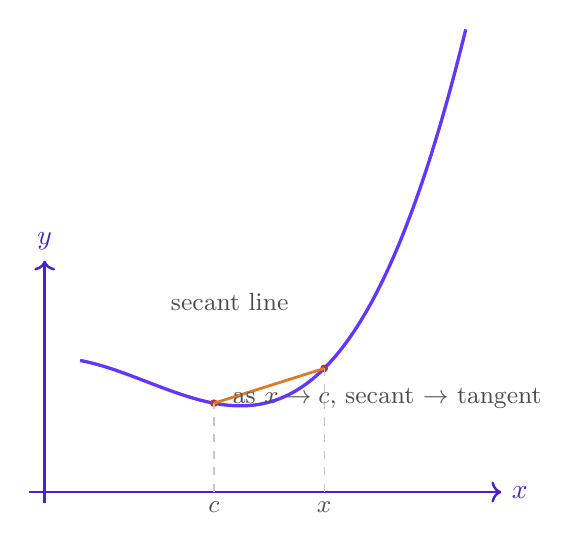
\begin{tikzpicture}[x=1cm,y=0.7cm]
\draw[novelPurpleDark, line width=0.9pt, ->] (-0.2,0)--(5.8,0) node[right] {$x$};
\draw[novelPurpleDark, line width=0.9pt, ->] (0,-0.2)--(0,4.2) node[above] {$y$};
\draw[novelPurple, line width=1.2pt, smooth, samples=240, domain=0.45:5.35]
plot (\x,{0.13*(\x-1.3)^3-0.55*(\x-1.3)+2.0});
\pgfmathsetmacro{\c}{2.15}
\pgfmathsetmacro{\d}{3.55}
\pgfmathsetmacro{\yc}{0.13*(\c-1.3)^3-0.55*(\c-1.3)+2.0}
\pgfmathsetmacro{\yd}{0.13*(\d-1.3)^3-0.55*(\d-1.3)+2.0}
\fill[npred] (\c,\yc) circle (1.4pt);
\fill[npred] (\d,\yd) circle (1.4pt);
\draw[gray!45,dashed] (\c,0)--(\c,\yc);
\draw[gray!45,dashed] (\d,0)--(\d,\yd);
\draw[nporange, line width=1.0pt] (\c,\yc)--(\d,\yd);
\node[text=npgray] at (2.35,3.45) {\small secant line};
\node[text=npgray] at (2.15,-0.28) {\small $c$};
\node[text=npgray] at (3.55,-0.28) {\small $x$};
\node[text=npgray] at (4.35,1.7) {\small as $x\to c$, secant $\to$ tangent};
\end{tikzpicture}
\end{center}
}

\newcommand{\rocfigure}{
\begin{center}
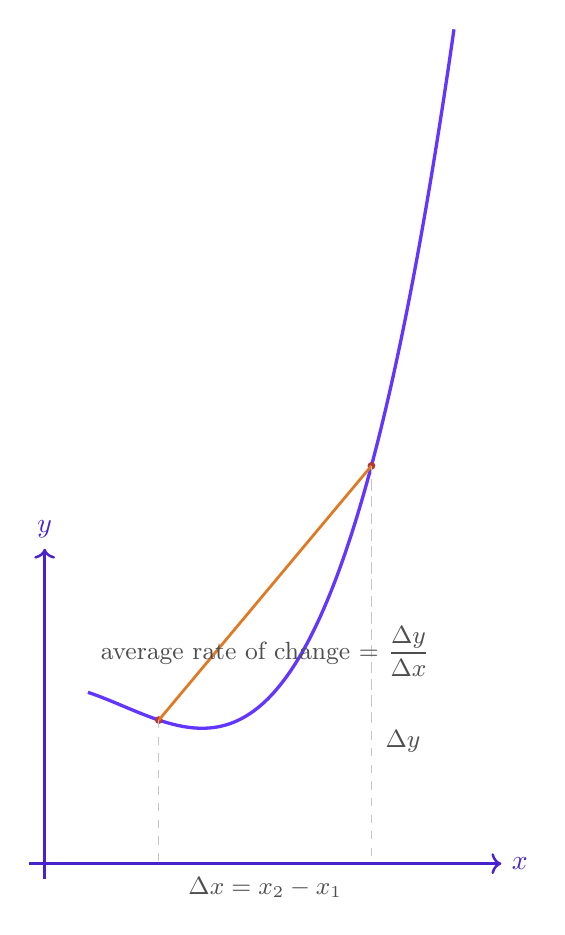
\begin{tikzpicture}[x=1cm,y=1cm]
\draw[novelPurpleDark, line width=0.9pt, ->] (-0.2,0)--(5.8,0) node[right] {$x$};
\draw[novelPurpleDark, line width=0.9pt, ->] (0,-0.2)--(0,4.0) node[above] {$y$};
\draw[novelPurple, line width=1.2pt, smooth, samples=220, domain=0.55:5.2]
plot (\x,{0.14*(\x-1.0)^3-0.42*(\x-1.0)+2.0});
\pgfmathsetmacro{\xone}{1.45}
\pgfmathsetmacro{\xtwo}{4.15}
\pgfmathsetmacro{\yone}{0.14*(\xone-1.0)^3-0.42*(\xone-1.0)+2.0}
\pgfmathsetmacro{\ytwo}{0.14*(\xtwo-1.0)^3-0.42*(\xtwo-1.0)+2.0}
\fill[npred] (\xone,\yone) circle (1.4pt);
\fill[npred] (\xtwo,\ytwo) circle (1.4pt);
\draw[nporange, line width=1.0pt] (\xone,\yone)--(\xtwo,\ytwo);
\draw[gray!45,dashed] (\xone,\yone)--(\xone,0);
\draw[gray!45,dashed] (\xtwo,\ytwo)--(\xtwo,0);
\draw[gray!45,dashed] (\xtwo,\yone)--(\xtwo,\ytwo);
\node[text=npgray] at (2.8,2.7) {\small average rate of change = $\dfrac{\Delta y}{\Delta x}$};
\node[text=npgray] at (2.8,-0.3) {\small $\Delta x=x_2-x_1$};
\node[text=npgray] at (4.55,1.55) {\small $\Delta y$};
\end{tikzpicture}
\end{center}
}



\newcommand{\tangentlimitsequencefigure}{
\begin{center}
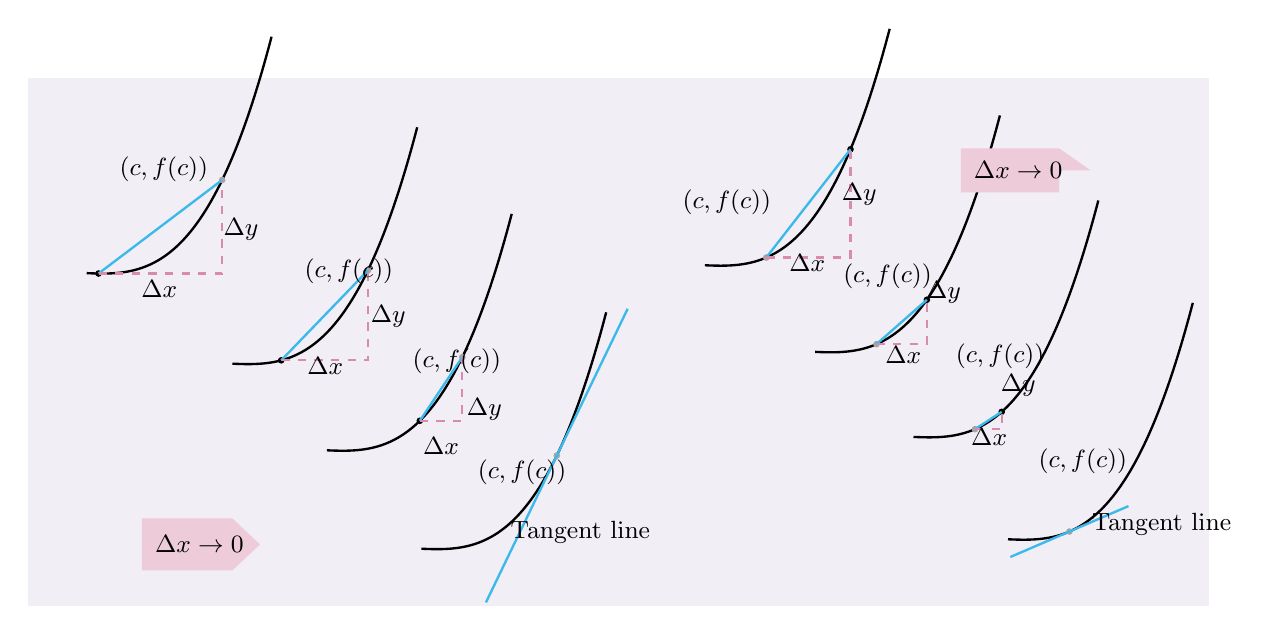
\begin{tikzpicture}[x=1cm,y=1cm,>=Latex]

% ---------- colors ----------
\definecolor{seqbg}{RGB}{241,238,245}      % pale lavender-gray
\definecolor{seqpink}{RGB}{214,140,170}
\definecolor{seqblue}{RGB}{60,185,235}
\definecolor{seqgray}{RGB}{165,165,165}

% ---------- background ----------
\fill[seqbg] (-0.4,-0.2) rectangle (14.6,6.5);

% =========================================================
% helper curve: y = 0.18(x-0.2)^2 + 0.22(x-0.2)^3 + 0.02
% tangent slope: y' = 0.36(x-0.2) + 0.66(x-0.2)^2
% =========================================================

% =========================================================
% LEFT GROUP  (Q approaches P from the left)
% =========================================================

% panel L1
\begin{scope}[shift={(0.35,4.0)}]
    \draw[black, line width=0.85pt, smooth, samples=200, domain=0:2.35]
        plot (\x,{0.18*(\x-0.2)^2 + 0.22*(\x-0.2)^3 + 0.02});

    \pgfmathsetmacro{\xp}{1.72}
    \pgfmathsetmacro{\yp}{0.18*(\xp-0.2)^2 + 0.22*(\xp-0.2)^3 + 0.02}
    \pgfmathsetmacro{\xq}{0.15}
    \pgfmathsetmacro{\yq}{0.18*(\xq-0.2)^2 + 0.22*(\xq-0.2)^3 + 0.02}

    \fill[black] (\xq,\yq) circle (1.2pt);
    \fill[seqgray] (\xp,\yp) circle (1.2pt);

    % true secant through P and Q
    \draw[seqblue, line width=0.85pt] (\xq,\yq)--(\xp,\yp);

    % delta box
    \draw[seqpink, dashed, line width=0.8pt] (\xq,\yq)--(\xp,\yq)--(\xp,\yp);
    \node at (0.92,-0.18) {\small $\Delta x$};
    \node at (1.96,0.58) {\small $\Delta y$};
    \node at (0.98,1.35) {\small $(c,f(c))$};
\end{scope}

% panel L2
\begin{scope}[shift={(2.2,2.85)}]
    \draw[black, line width=0.85pt, smooth, samples=200, domain=0:2.35]
        plot (\x,{0.18*(\x-0.2)^2 + 0.22*(\x-0.2)^3 + 0.02});

    \pgfmathsetmacro{\xp}{1.72}
    \pgfmathsetmacro{\yp}{0.18*(\xp-0.2)^2 + 0.22*(\xp-0.2)^3 + 0.02}
    \pgfmathsetmacro{\xq}{0.62}
    \pgfmathsetmacro{\yq}{0.18*(\xq-0.2)^2 + 0.22*(\xq-0.2)^3 + 0.02}

    \fill[black] (\xq,\yq) circle (1.2pt);
    \fill[seqgray] (\xp,\yp) circle (1.2pt);

    \draw[seqblue, line width=0.85pt] (\xq,\yq)--(\xp,\yp);

    \draw[seqpink, dashed, line width=0.8pt] (\xq,\yq)--(\xp,\yq)--(\xp,\yp);
    \node at (1.18,0.00) {\small $\Delta x$};
    \node at (1.98,0.62) {\small $\Delta y$};
    \node at (1.48,1.2) {\small $(c,f(c))$};
\end{scope}

% panel L3
\begin{scope}[shift={(3.4,1.75)}]
    \draw[black, line width=0.85pt, smooth, samples=200, domain=0:2.35]
        plot (\x,{0.18*(\x-0.2)^2 + 0.22*(\x-0.2)^3 + 0.02});

    \pgfmathsetmacro{\xp}{1.72}
    \pgfmathsetmacro{\yp}{0.18*(\xp-0.2)^2 + 0.22*(\xp-0.2)^3 + 0.02}
    \pgfmathsetmacro{\xq}{1.18}
    \pgfmathsetmacro{\yq}{0.18*(\xq-0.2)^2 + 0.22*(\xq-0.2)^3 + 0.02}

    \fill[black] (\xq,\yq) circle (1.2pt);
    \fill[seqgray] (\xp,\yp) circle (1.2pt);

    \draw[seqblue, line width=0.85pt] (\xq,\yq)--(\xp,\yp);

    \draw[seqpink, dashed, line width=0.8pt] (\xq,\yq)--(\xp,\yq)--(\xp,\yp);
    \node at (1.45,0.08) {\small $\Delta x$};
    \node at (2.00,0.55) {\small $\Delta y$};
    \node at (1.65,1.15) {\small $(c,f(c))$};
\end{scope}

% panel L4 tangent
\begin{scope}[shift={(4.6,0.5)}]
    \draw[black, line width=0.85pt, smooth, samples=200, domain=0:2.35]
        plot (\x,{0.18*(\x-0.2)^2 + 0.22*(\x-0.2)^3 + 0.02});

    \pgfmathsetmacro{\xp}{1.72}
    \pgfmathsetmacro{\yp}{0.18*(\xp-0.2)^2 + 0.22*(\xp-0.2)^3 + 0.02}
    \pgfmathsetmacro{\m}{0.36*(\xp-0.2) + 0.66*(\xp-0.2)^2}

    \fill[seqgray] (\xp,\yp) circle (1.2pt);

    % true tangent line
    \draw[seqblue, line width=0.85pt]
        ({\xp-0.9},{\yp-\m*0.9}) -- ({\xp+0.9},{\yp+\m*0.9});

    \node at (1.28,1.0) {\small $(c,f(c))$};
    \node at (2.02,0.23) {\small Tangent line};
\end{scope}

% left arrow
\fill[seqpink!45] (1.05,0.25) -- (2.20,0.25) -- (2.55,0.58) -- (2.20,0.91) -- (1.05,0.91) -- cycle;
\node at (1.78,0.58) {\small $\Delta x \to 0$};

% =========================================================
% RIGHT GROUP  (Q approaches P from the right)
% =========================================================

% panel R1
\begin{scope}[shift={(8.2,4.1)}]
    \draw[black, line width=0.85pt, smooth, samples=200, domain=0:2.35]
        plot (\x,{0.18*(\x-0.2)^2 + 0.22*(\x-0.2)^3 + 0.02});

    \pgfmathsetmacro{\xp}{0.78}
    \pgfmathsetmacro{\yp}{0.18*(\xp-0.2)^2 + 0.22*(\xp-0.2)^3 + 0.02}
    \pgfmathsetmacro{\xq}{1.85}
    \pgfmathsetmacro{\yq}{0.18*(\xq-0.2)^2 + 0.22*(\xq-0.2)^3 + 0.02}

    \fill[seqgray] (\xp,\yp) circle (1.2pt);
    \fill[black] (\xq,\yq) circle (1.2pt);

    \draw[seqblue, line width=0.85pt] (\xp,\yp)--(\xq,\yq);

    \draw[seqpink, dashed, line width=0.8pt] (\xp,\yp)--(\xq,\yp)--(\xq,\yq);
    \node at (1.30,0.06) {\small $\Delta x$};
    \node at (1.96,0.92) {\small $\Delta y$};
    \node at (0.28,0.82) {\small $(c,f(c))$};
\end{scope}

% panel R2
\begin{scope}[shift={(9.6,3.0)}]
    \draw[black, line width=0.85pt, smooth, samples=200, domain=0:2.35]
        plot (\x,{0.18*(\x-0.2)^2 + 0.22*(\x-0.2)^3 + 0.02});

    \pgfmathsetmacro{\xp}{0.78}
    \pgfmathsetmacro{\yp}{0.18*(\xp-0.2)^2 + 0.22*(\xp-0.2)^3 + 0.02}
    \pgfmathsetmacro{\xq}{1.42}
    \pgfmathsetmacro{\yq}{0.18*(\xq-0.2)^2 + 0.22*(\xq-0.2)^3 + 0.02}

    \fill[seqgray] (\xp,\yp) circle (1.2pt);
    \fill[black] (\xq,\yq) circle (1.2pt);

    \draw[seqblue, line width=0.85pt] (\xp,\yp)--(\xq,\yq);

    \draw[seqpink, dashed, line width=0.8pt] (\xp,\yp)--(\xq,\yp)--(\xq,\yq);
    \node at (1.12,-0.02) {\small $\Delta x$};
    \node at (1.63,0.78) {\small $\Delta y$};
    \node at (0.92,0.98) {\small $(c,f(c))$};
\end{scope}

% panel R3
\begin{scope}[shift={(10.85,1.92)}]
    \draw[black, line width=0.85pt, smooth, samples=200, domain=0:2.35]
        plot (\x,{0.18*(\x-0.2)^2 + 0.22*(\x-0.2)^3 + 0.02});

    \pgfmathsetmacro{\xp}{0.78}
    \pgfmathsetmacro{\yp}{0.18*(\xp-0.2)^2 + 0.22*(\xp-0.2)^3 + 0.02}
    \pgfmathsetmacro{\xq}{1.12}
    \pgfmathsetmacro{\yq}{0.18*(\xq-0.2)^2 + 0.22*(\xq-0.2)^3 + 0.02}

    \fill[seqgray] (\xp,\yp) circle (1.2pt);
    \fill[black] (\xq,\yq) circle (1.2pt);

    \draw[seqblue, line width=0.85pt] (\xp,\yp)--(\xq,\yq);

    \draw[seqpink, dashed, line width=0.8pt] (\xp,\yp)--(\xq,\yp)--(\xq,\yq);
    \node at (0.96,0.02) {\small $\Delta x$};
    \node at (1.33,0.68) {\small $\Delta y$};
    \node at (1.10,1.05) {\small $(c,f(c))$};
\end{scope}

% panel R4 tangent
\begin{scope}[shift={(12.05,0.62)}]
    \draw[black, line width=0.85pt, smooth, samples=200, domain=0:2.35]
        plot (\x,{0.18*(\x-0.2)^2 + 0.22*(\x-0.2)^3 + 0.02});

    \pgfmathsetmacro{\xp}{0.78}
    \pgfmathsetmacro{\yp}{0.18*(\xp-0.2)^2 + 0.22*(\xp-0.2)^3 + 0.02}
    \pgfmathsetmacro{\m}{0.36*(\xp-0.2) + 0.66*(\xp-0.2)^2}

    \fill[seqgray] (\xp,\yp) circle (1.2pt);

    \draw[seqblue, line width=0.85pt]
        ({\xp-0.75},{\yp-\m*0.75}) -- ({\xp+0.75},{\yp+\m*0.75});

    \node at (0.95,1.02) {\small $(c,f(c))$};
    \node at (1.95,0.22) {\small Tangent line};
\end{scope}

% right arrow
\fill[seqpink!45] (11.45,5.05) -- (12.7,5.05) -- (12.7,5.33) -- (13.1,5.33) -- (12.7,5.61) -- (11.45,5.61) -- cycle;
\node at (12.18,5.33) {\small $\Delta x \to 0$};

\end{tikzpicture}
\end{center}
}

\newcommand{\diffcontinuityfigure}{
\begin{center}
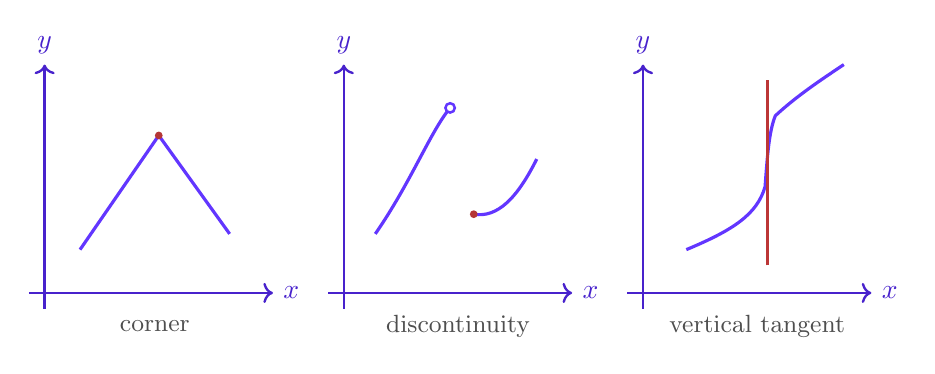
\begin{tikzpicture}[x=1cm,y=1cm]

% =========================
% 1. corner
% =========================
\begin{scope}[shift={(0,0)}]
    \draw[novelPurpleDark, line width=0.85pt, ->] (-0.2,0)--(2.9,0) node[right] {$x$};
    \draw[novelPurpleDark, line width=0.85pt, ->] (0,-0.2)--(0,2.9) node[above] {$y$};

    % actual corner
    \draw[novelPurple, line width=1.15pt]
        (0.45,0.55) -- (1.45,2.0) -- (2.35,0.75);

    \fill[npred] (1.45,2.0) circle (1.4pt);
    \node[text=npgray] at (1.4,-0.42) {\small corner};
\end{scope}

% =========================
% 2. discontinuity
% =========================
\begin{scope}[shift={(3.8,0)}]
    \draw[novelPurpleDark, line width=0.85pt, ->] (-0.2,0)--(2.9,0) node[right] {$x$};
    \draw[novelPurpleDark, line width=0.85pt, ->] (0,-0.2)--(0,2.9) node[above] {$y$};

    % left branch
    \draw[novelPurple, line width=1.15pt, smooth]
        (0.4,0.75) .. controls (0.85,1.4) and (1.1,2.05) .. (1.35,2.35);

    % right branch
    \draw[novelPurple, line width=1.15pt, smooth]
        (1.65,1.0) .. controls (1.95,0.95) and (2.2,1.2) .. (2.45,1.7);

    % open and closed dots
    \filldraw[white,draw=novelPurple,line width=0.9pt] (1.35,2.35) circle (1.7pt);
    \fill[npred] (1.65,1.0) circle (1.4pt);

    \node[text=npgray] at (1.45,-0.42) {\small discontinuity};
\end{scope}

% =========================
% 3. vertical tangent
% =========================
% =========================
% 3. vertical tangent
% =========================
\begin{scope}[shift={(7.6,0)}]
    \draw[novelPurpleDark, line width=0.85pt, ->] (-0.2,0)--(2.9,0) node[right] {$x$};
    \draw[novelPurpleDark, line width=0.85pt, ->] (0,-0.2)--(0,2.9) node[above] {$y$};

    % curve with a genuinely vertical-looking tangent in the middle
    \draw[novelPurple, line width=1.15pt]
        (0.55,0.55)
        .. controls (1.15,0.8) and (1.45,1.0) .. (1.55,1.35)
        .. controls (1.58,1.75) and (1.60,2.05) .. (1.68,2.25)
        .. controls (1.95,2.5) and (2.25,2.7) .. (2.55,2.9);

    % vertical tangent marker through the tangency point
    \draw[warmred, line width=0.9pt] (1.58,0.35)--(1.58,2.7);

    \node[text=npgray] at (1.45,-0.42) {\small vertical tangent};
\end{scope}

\end{tikzpicture}
\end{center}
}


\newcommand{\ruleflowfigure}{
\begin{center}
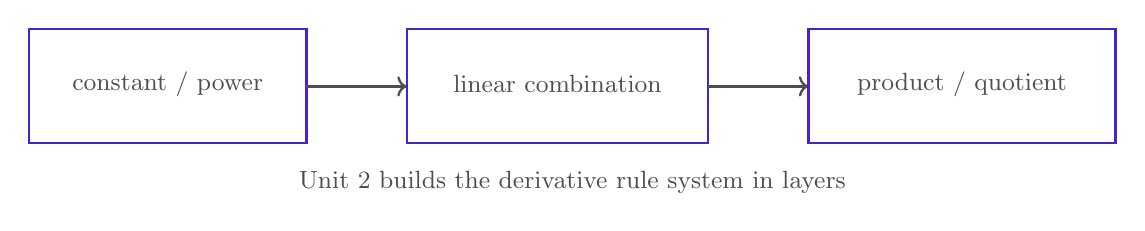
\begin{tikzpicture}[x=1.5cm,y=1cm]
\draw[novelPurpleDark, line width=0.9pt] (0,0) rectangle (2.35,1.45);
\node[text=npgray] at (1.175,0.75) {\small constant / power};
\draw[->, line width=0.85pt, npgray] (2.35,0.72)--(3.2,0.72);
\draw[novelPurpleDark, line width=0.9pt] (3.2,0) rectangle (5.75,1.45);
\node[text=npgray] at (4.475,0.75) {\small linear combination};
\draw[->, line width=0.85pt, npgray] (5.75,0.72)--(6.6,0.72);
\draw[novelPurpleDark, line width=0.9pt] (6.6,0) rectangle (9.2,1.45);
\node[text=npgray] at (7.9,0.75) {\small product / quotient};
\node[text=npgray] at (4.6,-0.5) {\small Unit 2 builds the derivative rule system in layers};
\end{tikzpicture}
\end{center}
}

\newcommand{\trigderivfigure}{
\begin{center}
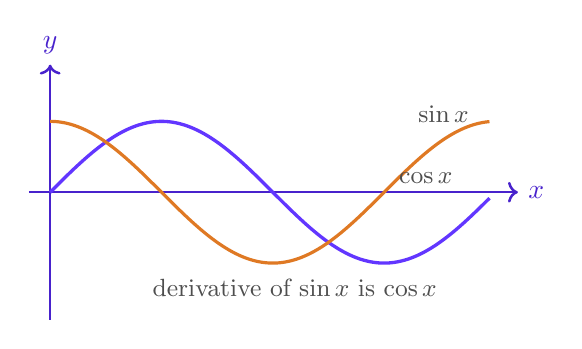
\begin{tikzpicture}[x=0.9cm,y=0.9cm]
\draw[novelPurpleDark, line width=0.9pt, ->] (-0.3,0)--(6.6,0) node[right] {$x$};
\draw[novelPurpleDark, line width=0.9pt, ->] (0,-1.8)--(0,1.8) node[above] {$y$};
\draw[novelPurple, line width=1.2pt, smooth, samples=220, domain=0:6.2]
plot (\x,{sin(deg(\x))});
\draw[nporange, line width=1.15pt, smooth, samples=220, domain=0:6.2]
plot (\x,{cos(deg(\x))});
\node[text=npgray] at (5.55,1.1) {\small $\sin x$};
\node[text=npgray] at (5.3,0.2) {\small $\cos x$};
\node[text=npgray] at (3.45,-1.35) {\small derivative of $\sin x$ is $\cos x$};
\end{tikzpicture}
\end{center}
}

\newcommand{\higherordercyclefigure}{
\begin{center}
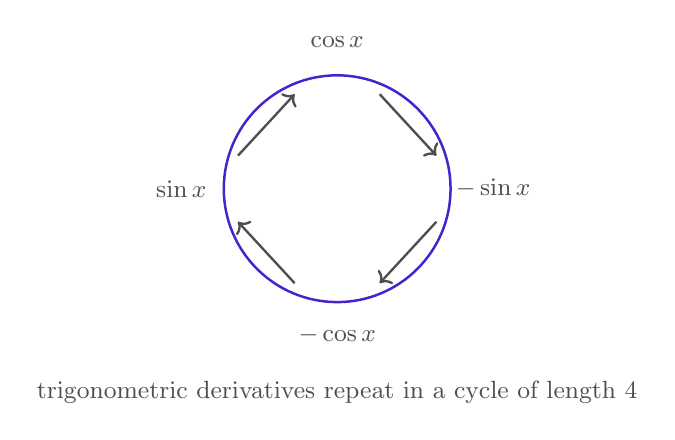
\begin{tikzpicture}[x=1.2cm,y=1.2cm]
\draw[novelPurpleDark, line width=0.9pt] (0,0) circle (1.2);
\node[text=npgray] at (0,1.55) {\small $\cos x$};
\node[text=npgray] at (1.65,0) {\small $-\sin x$};
\node[text=npgray] at (0,-1.55) {\small $-\cos x$};
\node[text=npgray] at (-1.65,0) {\small $\sin x$};
\draw[->, line width=0.85pt, npgray] (0.45,1.0)--(1.05,0.35);
\draw[->, line width=0.85pt, npgray] (1.05,-0.35)--(0.45,-1.0);
\draw[->, line width=0.85pt, npgray] (-0.45,-1.0)--(-1.05,-0.35);
\draw[->, line width=0.85pt, npgray] (-1.05,0.35)--(-0.45,1.0);
\node[text=npgray] at (0,-2.15) {\small trigonometric derivatives repeat in a cycle of length 4};
\end{tikzpicture}
\end{center}
}

% =========================
% Document
% =========================
\begin{document}

\begin{titlepage}
\centering
\vspace*{1.9cm}

{\fontsize{28}{32}\selectfont\bfseries\color{novelPurpleDark} AP Calculus AB\par}
\vspace{0.35cm}
{\fontsize{28}{32}\selectfont\bfseries\color{novelPurpleDark} Unit 2: Differentiation --- Definition and Fundamental Properties\par}


\vspace{1.0cm}
\unittwocoverfigure

\vfill

\begin{minipage}{0.84\textwidth}
\begin{notebox}{Design Goals for This Revision}
\begin{itemize}
    \item Preserve the original Unit 2 flow: tangent line problem, rate of change, the derivative definition, differentiability and continuity, basic rules, product and quotient rules, and trigonometric derivatives.
    \item Rebuild the chapter in the same polished Novel Prep style used for the optimized later units.
    \item Keep the original theorem path and representative examples while improving explanation, visual structure, and page rhythm.
    \item Add enough interpretation that students understand what a derivative means before they memorize rules.
    \item Make the chapter strong enough for both first instruction and AP Calculus AB review.
\end{itemize}
\end{notebox}
\end{minipage}

\vfill
{\large\textbf{Novel Prep Learning Center}}\\[0.25em]
{\large J. Z}

\end{titlepage}

\tableofcontents
\newpage

\setcounter{section}{1}
\section{Differentiation: Definition and Fundamental Properties}

\begin{theorybox}{Big Idea}
Unit 2 takes the idea of a limit and turns it into the derivative.
At first, the derivative is a slope and an instantaneous rate of change.
Then, once that meaning is secure, the chapter builds a complete toolkit of differentiation rules.
\end{theorybox}

\begin{notebox}{Teaching Philosophy for This Unit}
Students should not experience Unit 2 as a list of formulas.
The chapter has a natural progression:
\[
\text{secant slope} \longrightarrow \text{tangent slope} \longrightarrow \text{derivative definition} \longrightarrow \text{derivative rules}.
\]
Once students understand that all of the rules are shortcuts built from the same limit idea, the chapter becomes much more coherent.
\end{notebox}

\begin{summarybox}{AP Checkpoint}
By the end of Unit 2, students should be able to:
\begin{itemize}
    \item interpret the derivative geometrically and contextually,
    \item compute derivatives from the limit definition in basic cases,
    \item explain why differentiability implies continuity,
    \item use constant, power, sum, difference, product, and quotient rules,
    \item and differentiate the standard trigonometric functions.
\end{itemize}
\end{summarybox}

% =========================================================
\unitchapter{The Derivative and the Tangent Line Problem}

\unitsubtopic{The Tangent Line Problem}

\begin{theorybox}{Definition 2.1.1 --- Tangent Line with Slope $m$}
If $f$ is defined on an open interval containing $c$, and if the limit
\[
\lim_{\Delta x\to 0}\frac{\Delta y}{\Delta x}
=\lim_{\Delta x\to0}\frac{f(c+\Delta x)-f(c)}{\Delta x}
\]
exists, then the line passing through $(c,f(c))$ with slope $m$ is the tangent line to the graph of $f$ at the point $(c,f(c))$.
\end{theorybox}

\tangentlimitfigure

\tangentlimitsequencefigure


\begin{summarybox}{Core Geometric Meaning}
The slope of the tangent line to the graph of $f$ at $(c,f(c))$ is also called the slope of the graph at $x=c$.
The tangent line is the limit position of secant lines as the second point moves toward the first.
\end{summarybox}

\example{The slope of the graph of a linear function}
Use the tangent-line definition to find the slope of the graph of
\[
f(x)=2x-3
\]
when $c=2$.

\solution
By definition,
\[
\lim_{\Delta x\to0}\frac{f(2+\Delta x)-f(2)}{\Delta x}
=\lim_{\Delta x\to0}\frac{[2(2+\Delta x)-3]-[2(2)-3]}{\Delta x}.
\]
Simplify:
\[
=\lim_{\Delta x\to0}\frac{4+2\Delta x-3-4+3}{\Delta x}
=\lim_{\Delta x\to0}\frac{2\Delta x}{\Delta x}
=\lim_{\Delta x\to0}2=2.
\]
Thus the slope is
\[
\boxed{2}.
\]
This confirms that for a linear function, the tangent slope is the constant slope of the line itself.

\unitsubtopic{Rate of Change}

\begin{theorybox}{Definition 2.1.2 --- Rate of Change}
Suppose $y=f(x)$. If $x$ changes from $x_1$ to $x_2$, then
\[
\Delta x=x_2-x_1,
\qquad
\Delta y=f(x_2)-f(x_1).
\]
The quotient
\[
\frac{\Delta y}{\Delta x}=\frac{f(x_2)-f(x_1)}{x_2-x_1}
\]
is the average rate of change of $y$ with respect to $x$ over $[x_1,x_2]$.
Its limit is the instantaneous rate of change:
\[
\lim_{\Delta x\to0}\frac{\Delta y}{\Delta x}=
\lim_{x_2\to x_1}\frac{f(x_2)-f(x_1)}{x_2-x_1}.
\]
\end{theorybox}

\rocfigure

\begin{notebox}{Teacher Emphasis}
Average rate of change uses two points and gives a secant slope.
Instantaneous rate of change uses a limit and gives a tangent slope.
Students should see these as the same idea at two different scales.
\end{notebox}

\example{Understanding the derivative in a practical context}
A manufacturer produces bolts of fabric with fixed width. The cost of producing $x$ yards is $C=f(x)$ dollars.
What is the meaning of $f'(x)$? What are its units?

\solution
The derivative $f'(x)$ is the instantaneous rate of change of production cost with respect to the number of yards produced.
Economically, this is the \textbf{marginal cost}.

In symbols,
\[
f'(x)=\lim_{\Delta x\to0}\frac{\Delta C}{\Delta x}.
\]
Since $\Delta C$ is measured in dollars and $\Delta x$ in yards, the units of $f'(x)$ are
\[
\boxed{\text{dollars per yard}.}
\]

\unitsubtopic{The Derivative of a Function}

\begin{theorybox}{Definition 2.1.3 --- The Derivative of a Function}
The derivative of $f$ at $x$ is
\[
f'(x)=\lim_{\Delta x\to0}\frac{f(x+\Delta x)-f(x)}{\Delta x}
\]
provided the limit exists. For all $x$ where the limit exists, $f'$ is itself a function of $x$.
\end{theorybox}

\begin{summarybox}{Equivalent Notation}
You may also see the derivative written as
\[
f'(x),\qquad y',\qquad \frac{dy}{dx},\qquad \frac{d}{dx}[f(x)].
\]
These all refer to the same derivative idea, but the best notation depends on context.
\end{summarybox}

\example{Finding the derivative from the definition}
Find the derivative of
\[
f(x)=x^3+2x
\]
using the definition.

\solution
Start with
\[
f'(x)=\lim_{h\to0}\frac{f(x+h)-f(x)}{h}.
\]
Compute:
\[
f(x+h)=(x+h)^3+2(x+h)=x^3+3x^2h+3xh^2+h^3+2x+2h.
\]
So
\[
f'(x)=\lim_{h\to0}\frac{x^3+3x^2h+3xh^2+h^3+2x+2h-x^3-2x}{h}.
\]
Simplify:
\[
=\lim_{h\to0}\frac{3x^2h+3xh^2+h^3+2h}{h}
=\lim_{h\to0}(3x^2+3xh+h^2+2).
\]
Now take the limit:
\[
\boxed{f'(x)=3x^2+2.}
\]

\unitsubtopic{Differentiability and Continuity}

\begin{theorybox}{Definition 2.1.4 --- Differentiability and Continuity}
A function $f$ is differentiable at $a$ if $f'(a)$ exists.
It is differentiable on an interval if it is differentiable at every point in the interval.
\end{theorybox}

\begin{summarybox}{Important Relationship}
If a function is differentiable at a point, then it must be continuous there.
However, continuity alone does not guarantee differentiability.
\end{summarybox}

\diffcontinuityfigure

\begin{notebox}{How a Function Can Fail To Be Differentiable}
A function may fail to be differentiable at $x=a$ because of:
\begin{enumerate}
    \item a corner or kink,
    \item a discontinuity,
    \item a vertical tangent line.
\end{enumerate}
These match the three standard AP graph-based cases.
\end{notebox}

\example{A graph with a sharp turn}
Show that
\[
f(x)=|x-2|
\]
is not differentiable at $x=2$.

\solution
Since $f(2)=0$,
\[
\lim_{x\to2^-}\frac{f(x)-f(2)}{x-2}
=\lim_{x\to2^-}\frac{|x-2|}{x-2}=-1.
\]
But
\[
\lim_{x\to2^+}\frac{f(x)-f(2)}{x-2}
=\lim_{x\to2^+}\frac{|x-2|}{x-2}=1.
\]
The one-sided derivatives are not equal, so $f$ is not differentiable at $x=2$.
Thus,
\[
\boxed{f \text{ is continuous at } x=2 \text{ but not differentiable there.}}
\]

\example{A graph with a vertical tangent line}
Explain why
\[
f(x)=x^{1/3}
\]
is not differentiable at $x=0$.

\solution
Use the derivative definition at $x=0$:
\[
\lim_{x\to0}\frac{f(x)-f(0)}{x-0}
=\lim_{x\to0}\frac{x^{1/3}}{x}
=\lim_{x\to0}\frac{1}{x^{2/3}}.
\]
This limit becomes infinite, so the tangent line is vertical at $x=0$.
Therefore,
\[
\boxed{f \text{ is not differentiable at } x=0.}
\]

% =========================================================
\unitchapter{Basic Differentiation Rules}

\begin{summarybox}{Why Rules Matter}
The limit definition is foundational, but it is not efficient for every problem.
The rules in this section are shortcuts built from the same derivative idea.
Once students trust the definition, these rules become natural tools rather than isolated facts.
\end{summarybox}

\ruleflowfigure

\unitsubtopic{The Constant Rule}

\begin{theorybox}{Theorem 2.2.1 --- The Constant Rule}
If $c$ is a real number, then
\[
\frac{d}{dx}[c]=0.
\]
\end{theorybox}

\example{Using the constant rule}
Differentiate each function.
\begin{enumerate}
    \item $y=7$
    \item $f(x)=0$
    \item $s(t)=-3$
    \item $y=k\pi^2$ where $k$ is constant
\end{enumerate}

\solution
Each derivative is zero because the function never changes:
\[
\boxed{y'=0,\quad f'(x)=0,\quad s'(t)=0,\quad y'=0.}
\]

\unitsubtopic{The Power Rule}

\begin{theorybox}{Theorem 2.2.2 --- Power Rule}
If $n$ is a rational number, then
\[
\frac{d}{dx}[x^n]=nx^{n-1}
\]
where the resulting expression is defined.
\end{theorybox}

\begin{notebox}{Teacher Emphasis}
The Power Rule covers positive powers, negative powers, and many rational powers.
Students should always check whether the resulting derivative is defined at the point of interest.
\end{notebox}

\example{Using the power rule}
Differentiate each function.
\begin{enumerate}
    \item $f(x)=x^3$
    \item $g(x)=x^{1/3}$
    \item $y=\dfrac{1}{x^2}$
\end{enumerate}

\solution
\textbf{(a)}
\[
f'(x)=3x^2.
\]

\textbf{(b)}
\[
g'(x)=\frac13x^{-2/3}=\frac{1}{3x^{2/3}}.
\]

\textbf{(c)} Rewrite first:
\[
y=x^{-2}.
\]
Then
\[
y'=(-2)x^{-3}=-\frac{2}{x^3}.
\]

\unitsubtopic{The Constant Multiple Rule}

\begin{theorybox}{Theorem 2.2.3 --- Constant Multiple Rule}
If $f$ is differentiable and $c$ is a real number, then
\[
\frac{d}{dx}[cf(x)]=cf'(x).
\]
\end{theorybox}

\example{Using the constant multiple rule}
Differentiate each function.
\begin{enumerate}
    \item $y=5x^3$
    \item $y=\dfrac{2}{x}$
    \item $f(t)=4t^2$
    \item $y=2\sqrt{x}$
\end{enumerate}

\solution
\[
\boxed{\frac{dy}{dx}=15x^2,\qquad \frac{dy}{dx}=-\frac{2}{x^2},\qquad f'(t)=8t,\qquad \frac{dy}{dx}=\frac{1}{\sqrt{x}}.}
\]

\unitsubtopic{The Sum and Difference Rules}

\begin{theorybox}{Theorem 2.2.4 --- Sum and Difference Rules}
If $f$ and $g$ are differentiable, then
\[
\frac{d}{dx}[f(x)+g(x)]=f'(x)+g'(x)
\]
and
\[
\frac{d}{dx}[f(x)-g(x)]=f'(x)-g'(x).
\]
\end{theorybox}

\example{Using the sum and difference rules}
Differentiate each function.
\begin{enumerate}
    \item $f(x)=x^3-4x+5$
    \item $g(x)=-\dfrac{x^4}{2}+3x^3-2x$
    \item $y=\dfrac{3x^2-x+1}{x}=3x-1+\dfrac1x$
\end{enumerate}

\solution
\textbf{(a)}
\[
f'(x)=3x^2-4.
\]

\textbf{(b)}
\[
g'(x)=-2x^3+9x^2-2.
\]

\textbf{(c)} Rewrite first:
\[
y=3x-1+x^{-1}.
\]
Then
\[
y'=3-x^{-2}=3-\frac{1}{x^2}=\frac{3x^2-1}{x^2}.
\]

\unitsubtopic{Derivatives of Sine and Cosine Functions}

\begin{theorybox}{Theorem 2.2.5 --- Derivatives of Sine and Cosine}
The derivatives of the sine and cosine functions are
\[
\frac{d}{dx}[\sin x]=\cos x,
\qquad
\frac{d}{dx}[\cos x]=-\sin x.
\]
\end{theorybox}

\trigderivfigure

\example{Derivatives of sine and cosine functions}
Differentiate each function.
\begin{enumerate}
    \item $y=2\sin x$
    \item $y=\dfrac{\sin x}{2}$
    \item $y=x+\cos x$
    \item $y=\cos x-\dfrac{\pi}{3}\sin x$
\end{enumerate}

\solution
\[
\boxed{y'=2\cos x,\qquad y'=\frac12\cos x,\qquad y'=1-\sin x,\qquad y'=-\sin x-\frac{\pi}{3}\cos x.}
\]

% =========================================================
\unitchapter{Product and Quotient Rules and Higher-Order Derivatives}

\begin{notebox}{Why New Rules Are Needed}
The derivative of a sum is easy to separate term-by-term.
Products and quotients are different: their derivatives are not simply the product or quotient of the derivatives.
That is why Unit 2 adds two new structural rules here.
\end{notebox}

\unitsubtopic{Product Rule}

\begin{theorybox}{Theorem 2.3.1 --- Product Rule}
If $f$ and $g$ are differentiable, then
\[
\frac{d}{dx}[f(x)g(x)] = f(x)g'(x)+g(x)f'(x).
\]
\end{theorybox}

\example{Using the product rule}
Differentiate
\[
f(t)=\sqrt{t}(a+bt).
\]

\solution
Apply the Product Rule:
\[
f'(t)=\sqrt{t}\,\frac{d}{dt}(a+bt)+(a+bt)\frac{d}{dt}(\sqrt{t}).
\]
Compute each derivative:
\[
\frac{d}{dt}(a+bt)=b,
\qquad
\frac{d}{dt}(\sqrt{t})=\frac{1}{2\sqrt{t}}.
\]
So
\[
f'(t)=b\sqrt{t}+\frac{a+bt}{2\sqrt{t}}.
\]
Combine over a common denominator:
\[
f'(t)=\frac{2bt+a+bt}{2\sqrt{t}}=\boxed{\frac{a+3bt}{2\sqrt{t}}.}
\]
\newpage
\unitsubtopic{Quotient Rule}

\begin{theorybox}{Theorem 2.3.2 --- Quotient Rule}
If $f$ and $g$ are differentiable and $g(x)\neq 0$, then
\[
\frac{d}{dx}\left[\frac{f(x)}{g(x)}\right]
=
\frac{g(x)f'(x)-f(x)g'(x)}{[g(x)]^2}.
\]
\end{theorybox}

\example{Using the quotient rule to find a tangent line}
Find an equation of the tangent line to
\[
y=\frac{e^x}{1+x^2}
\]
at the point
\[
\left(1,\frac{e}{2}\right).
\]

\solution
Use the Quotient Rule:
\[
\frac{dy}{dx}=rac{(1+x^2)e^x-e^x(2x)}{(1+x^2)^2}.
\]
Factor out $e^x$:
\[
\frac{dy}{dx}=rac{e^x(1-2x+x^2)}{(1+x^2)^2}.
\]
Now evaluate at $x=1$:
\[
\left.\frac{dy}{dx}\right|_{x=1}=rac{e(1-2+1)}{(2)^2}=0.
\]
So the tangent line is horizontal, and since the point is
\[
\left(1,\frac{e}{2}\right),
\]
the tangent line is
\[
\boxed{y=\frac{e}{2}}.
\]

\begin{summarybox}{Unit 2 Rule Table So Far}
\renewcommand{\arraystretch}{1.35}
\begin{tabularx}{\textwidth}{@{}p{0.42\textwidth}X@{}}
\toprule
\textbf{Formula} & \textbf{Rule}\\
\midrule
$\dfrac{d}{dx}(c)=0$ & Constant rule\\
$\dfrac{d}{dx}(x^n)=nx^{n-1}$ & Power rule\\
$\dfrac{d}{dx}[cf(x)]=cf'(x)$ & Constant multiple rule\\
$\dfrac{d}{dx}[f+g]=f'+g'$ & Sum rule\\
$\dfrac{d}{dx}[f-g]=f'-g'$ & Difference rule\\
$\dfrac{d}{dx}[fg]=f'g+fg'$ & Product rule\\
$\dfrac{d}{dx}\left(\dfrac{f}{g}\right)=\dfrac{gf'-fg'}{g^2}$ & Quotient rule\\
\bottomrule
\end{tabularx}
\end{summarybox}

% =========================================================
\unitchapter{Derivatives of Trigonometric Functions}

\begin{theorybox}{Note 2.4.1 --- Table of Trigonometric Derivatives}
\[
\frac{d}{dx}(\sin x)=\cos x,
\qquad
\frac{d}{dx}(\cos x)=-\sin x,
\]
\[
\frac{d}{dx}(\tan x)=\sec^2 x,
\qquad
\frac{d}{dx}(\cot x)=-\csc^2 x,
\]
\[
\frac{d}{dx}(\sec x)=\sec x\tan x,
\qquad
\frac{d}{dx}(\csc x)=-\csc x\cot x.
\]
\end{theorybox}

\begin{notebox}{Teacher Emphasis}
Students should memorize these as a connected family, not as six isolated facts.
A good habit is to pair them mentally:
\begin{itemize}
    \item $\sin \leftrightarrow \cos$
    \item $\tan \leftrightarrow \sec^2$
    \item $\cot \leftrightarrow -\csc^2$
    \item $\sec \leftrightarrow \sec\tan$
    \item $\csc \leftrightarrow -\csc\cot$
\end{itemize}
\end{notebox}

\example{Derivatives of trigonometric functions with a quotient}
Differentiate
\[
f(x)=\frac{\sec x}{1+\tan x}.
\]
For what values of $x$ does the graph of $f$ have a horizontal tangent?

\solution
Use the Quotient Rule:
\[
f'(x)=\frac{(1+\tan x)\,\dfrac{d}{dx}(\sec x)-\sec x\,\dfrac{d}{dx}(1+\tan x)}{(1+\tan x)^2}.
\]
Substitute derivatives:
\[
f'(x)=\frac{(1+\tan x)(\sec x\tan x)-\sec x(\sec^2 x)}{(1+\tan x)^2}.
\]
Factor out $\sec x$:
\[
f'(x)=\frac{\sec x(\tan x+\tan^2x-\sec^2x)}{(1+\tan x)^2}.
\]
Use the identity
\[
\sec^2x=1+\tan^2x.
\]
Then
\[
f'(x)=\frac{\sec x(\tan x-1)}{(1+\tan x)^2}.
\]
So the graph has a horizontal tangent when
\[
\tan x-1=0
\quad\Rightarrow\quad
\tan x=1.
\]
Thus,
\[
\boxed{x=\frac{\pi}{4}+k\pi,\quad k\in\mathbb{Z},}
\]
provided the original function is defined there.

\unitsubtopic{Higher-Order Derivatives in Trigonometric Functions}

\begin{theorybox}{Repeated Derivatives of Sine and Cosine}
The derivatives of sine and cosine repeat in cycles of length 4.
This makes high-order derivatives of trigonometric functions especially manageable.
\end{theorybox}

\higherordercyclefigure

\example{Find a high-order derivative of cosine}
Find the $27$th derivative of
\[
f(x)=\cos x.
\]

\solution
Differentiate repeatedly:
\[
f'(x)=-\sin x,
\qquad
f''(x)=-\cos x,
\qquad
f^{(3)}(x)=\sin x,
\qquad
f^{(4)}(x)=\cos x.
\]
The pattern repeats every 4 derivatives.
Since
\[
27\equiv 3\pmod 4,
\]
the $27$th derivative matches the third derivative in the cycle.
Therefore,
\[
\boxed{f^{(27)}(x)=\sin x.}
\]

% =========================================================
\newpage
\subsection{Unit 2 Summary / Formula Sheet}

\begin{summarybox}{Unit 2 Master Summary Sheet}
\renewcommand{\arraystretch}{1.35}
\begin{tabularx}{\textwidth}{@{}p{0.38\textwidth}X@{}}
\toprule
\textbf{Topic} & \textbf{Key Formula / Idea} \\
\midrule
Tangent slope & $\displaystyle m=\lim_{\Delta x\to0}\frac{f(c+\Delta x)-f(c)}{\Delta x}$ \\
Average rate of change & $\displaystyle \frac{f(x_2)-f(x_1)}{x_2-x_1}$ \\
Derivative definition & $\displaystyle f'(x)=\lim_{h\to0}\frac{f(x+h)-f(x)}{h}$ \\
Differentiability and continuity & differentiable $\Rightarrow$ continuous \\
Constant rule & $\dfrac{d}{dx}(c)=0$ \\
Power rule & $\dfrac{d}{dx}(x^n)=nx^{n-1}$ \\
Constant multiple rule & $\dfrac{d}{dx}[cf]=cf'$ \\
Sum / difference rules & $(f\pm g)'=f'\pm g'$ \\
Product rule & $(fg)'=f'g+fg'$ \\
Quotient rule & $\left(\dfrac{f}{g}\right)'=\dfrac{gf'-fg'}{g^2}$ \\
Trig derivatives & $\sin',\cos',\tan',\cot',\sec',\csc'$ \\
\bottomrule
\end{tabularx}
\end{summarybox}

\vspace{1em}

\begin{summarybox}{Big Strategy Ladder}
\begin{itemize}
    \item First interpret the derivative as a tangent slope or instantaneous rate of change.
    \item Then learn the derivative definition well enough to compute simple derivatives from first principles.
    \item After that, use derivative rules as efficient shortcuts.
    \item Finally, combine these rules with trigonometric functions and more complicated algebraic expressions.
\end{itemize}
\end{summarybox}

% =========================================================
\newpage
\subsection{Guided Practice Set}

\begin{practicebox}{Guided Practice A --- Meaning of the Derivative}
\begin{enumerate}
    \item Explain the difference between a secant line and a tangent line.
    \item Compute the average rate of change of $f(x)=x^2+1$ on $[1,3]$.
    \item Use the derivative definition to find the slope of $f(x)=3x+2$ at $x=1$.
    \item Explain why the derivative can be interpreted as an instantaneous rate of change.
\end{enumerate}
\end{practicebox}

\begin{practicebox}{Guided Practice B --- Limit Definition and Differentiability}
\begin{enumerate}
    \item Use the limit definition to find the derivative of $f(x)=x^2$.
    \item Determine whether $f(x)=|x|$ is differentiable at $x=0$.
    \item Explain why differentiability implies continuity.
    \item Give one example of a function that is continuous but not differentiable at a point.
\end{enumerate}
\end{practicebox}

\begin{practicebox}{Guided Practice C --- Rules and Trigonometric Derivatives}
\begin{enumerate}
    \item Differentiate $y=4x^3-2x+7$.
    \item Differentiate $y=(x^2+1)(x-3)$.
    \item Differentiate $y=\dfrac{x^2+1}{x}$.
    \item Differentiate $y=\sin x+2\cos x$.
\end{enumerate}
\end{practicebox}

% =========================================================
\newpage
\subsection{Homework / Class Exercises}

\begin{practicebox}{Level 1 --- Skill Check}
\begin{enumerate}
    \item Use the derivative definition to find the derivative of $f(x)=x^2+3x$.
    \item Find the average rate of change of $f(x)=x^3$ on $[1,2]$.
    \item Determine whether $f(x)=|x-2|$ is differentiable at $x=2$.
    \item Differentiate $y=7x^4-3x+5$.
    \item Differentiate $y=2\sin x-\cos x$.
\end{enumerate}
\end{practicebox}

\begin{practicebox}{Level 2 --- AP Style Practice}
\begin{enumerate}
    \setcounter{enumi}{5}
    \item Differentiate $y=(x^2+1)(x^3-2)$.
    \item Differentiate $y=\dfrac{e^x}{1+x^2}$.
    \item Find the equation of the tangent line to $y=\dfrac{e^x}{1+x^2}$ at $x=1$.
    \item For what values of $x$ does the graph of $f(x)=\dfrac{\sec x}{1+\tan x}$ have a horizontal tangent?
    \item Explain, using a graph-based argument, why a vertical tangent does not give differentiability.
\end{enumerate}
\end{practicebox}

\begin{practicebox}{Level 3 --- Challenge / Extension}
\begin{enumerate}
    \setcounter{enumi}{10}
    \item Show from the limit definition that the derivative of a constant function is 0.
    \item Find the derivative of $y=x^{1/3}$ and explain what happens at $x=0$.
    \item Find the $18$th derivative of $\sin x$.
    \item Find the derivative of $y=\dfrac{x^2-1}{x^2+1}$.
    \item Explain why product and quotient rules are necessary, rather than trying to differentiate each factor separately and multiply or divide.
\end{enumerate}
\end{practicebox}

% =========================================================
\newpage
\subsection{Answer Key / Instructor Notes}

\begin{summarybox}{Selected Answers}
\begin{enumerate}
    \item From the definition, $\dfrac{d}{dx}(x^2+3x)=2x+3$
    \item Average rate of change of $x^3$ on $[1,2]$ is $\dfrac{8-1}{2-1}=7$
    \item $|x-2|$ is not differentiable at $x=2$ because left and right derivatives are $-1$ and $1$
    \item $\dfrac{d}{dx}(7x^4-3x+5)=28x^3-3$
    \item $\dfrac{d}{dx}(2\sin x-\cos x)=2\cos x+\sin x$
    \item $\dfrac{d}{dx}[(x^2+1)(x^3-2)]=2x(x^3-2)+(x^2+1)(3x^2)$
    \item $\dfrac{d}{dx}\left(\dfrac{e^x}{1+x^2}\right)=\dfrac{e^x(1-2x+x^2)}{(1+x^2)^2}$
    \item At $x=1$, tangent line is horizontal, so $y=\dfrac{e}{2}$
    \item Horizontal tangents occur when $\tan x=1$, so $x=\dfrac{\pi}{4}+k\pi$
    \item A vertical tangent corresponds to an infinite slope, so the derivative does not exist as a finite number
\end{enumerate}
\end{summarybox}

% =========================================================
\newpage
\subsection{Unit 2 Final Teaching Checklist}

\begin{summarybox}{Before Leaving Unit 2, Students Should Comfortably Handle}
\begin{itemize}
    \item moving from secant slope to tangent slope conceptually
    \item computing and interpreting average and instantaneous rates of change
    \item using the derivative definition in straightforward algebraic cases
    \item distinguishing continuity from differentiability
    \item recognizing corners, discontinuities, and vertical tangents as standard non-differentiable cases
    \item applying the constant, power, constant multiple, sum, and difference rules quickly and accurately
    \item using the product and quotient rules in algebraic and exponential examples
    \item differentiating the six basic trigonometric functions
    \item recognizing cyclic patterns in higher-order trigonometric derivatives
    \item seeing Unit 2 as the conceptual foundation for every later unit in calculus
\end{itemize}
\end{summarybox}

\end{document}
